
%%% Local Variables: 
%%% mode: latex
%%% TeX-master: t
%%% End: 

\documentclass[twocolumn]{article}

% Packages
% \usepackage{fancyhdr}
\usepackage{amsmath}
\usepackage{amssymb}
\usepackage[margin=10mm]{geometry}
\usepackage{graphicx}



% Housekeeping
% Detailed study is your responsibility.
\pagestyle{empty}

\begin{document}

\begin{itemize}
\item As pointed out by your father, for the master degree here, you
  only have one more year. To be or not to be, it's pretty obvious.
\item The best worst-case running time for comparison sorting is
  $O(n\log n)$.
  \begin{figure}[!h]
    \centering
    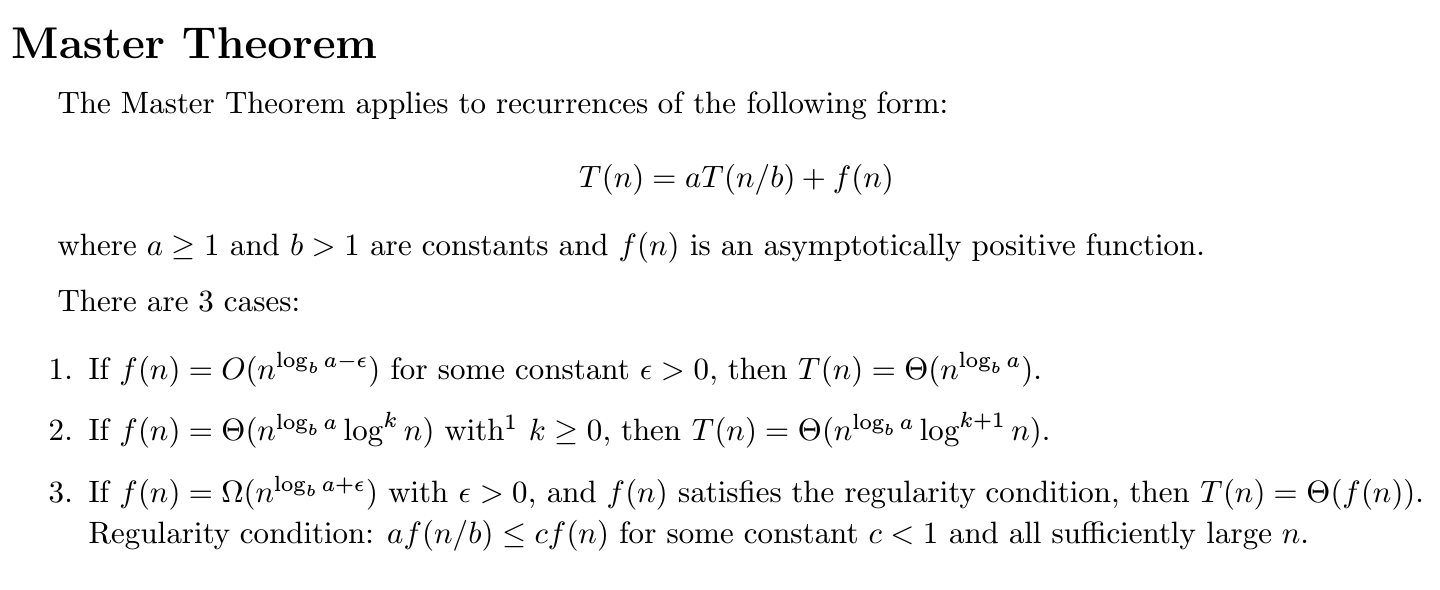
\includegraphics[scale=0.2]{snapshot95}
  \end{figure}
\item Given an open-address hash table with load factor $\alpha~=~n/m
  < 1$, the expected number of probes in an unsuccessfully search is
  \textbf{at most} $1/(1-\alpha)$, assuming uniform hashing.
  \begin{figure}[!h]
    \centering
    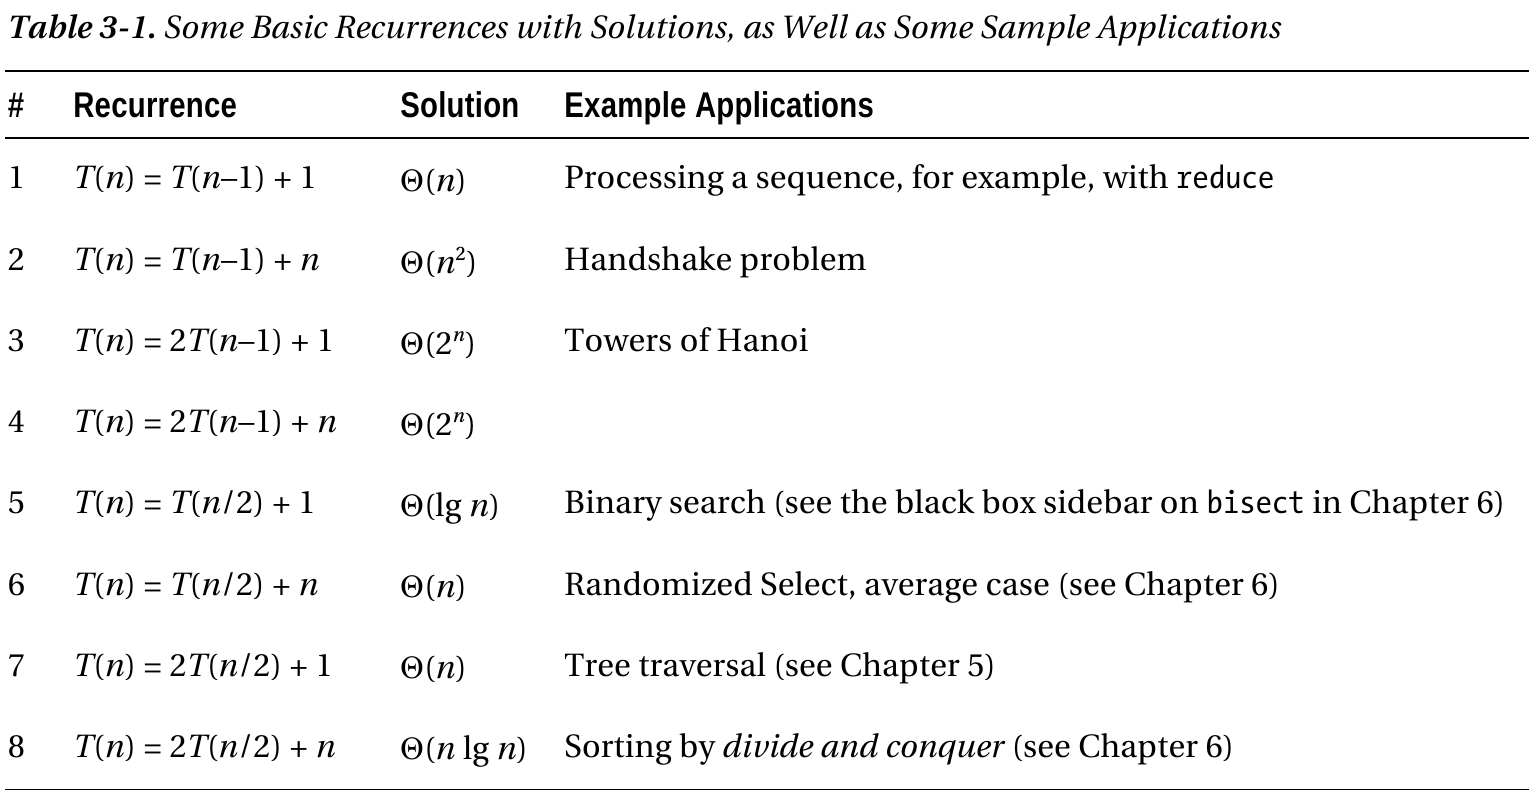
\includegraphics[scale=0.2]{snapshot96}
  \end{figure}
\end{itemize}

\end{document}
